% Checked with Grammarly - 22/03/2021

\chapter{Problem Analysis and Design Overview}

\section{Problem Analysis}

Preemptive botnet detection has often challenged authorities, as real-time, large-scale traffic analysis is often expensive and very difficult to coordinate. Current detection systems are often reactive, as they often rely on post-attack data sources and network logs from Internet Service Providers and DNS services. This approach is not ideal, as attacks must first take place to identify offending networks. The preemptive botnet detection technique proposed by \citet{Moon2012} proved significant in detecting botnets before attacks took place. The purposeful execution and analysis of malware enabled botnets to be identified and mitigated during their propagation periods. This system allows for the automatic collection and analysis of binaries using two dedicated processing modules. 

However, several issues are also presented within the detection framework proposed by Moon et al.. A primary concern is that the data collection methods employed are only achievable through integration with an Internet Service Provider (ISP) infrastructure. Thus, it isn't easy to reproduce the same data collection process without internal access to an ISP service. Additionally, the amount and type of information sourced from the KORNET ISP service varied significantly in scope and relevance to botnet propagation. The vast majority of binaries analysed were sourced from spam emails and malicious websites reported by KORNET users, with a significantly smaller number of binaries collected through botnet honeypots. The analysis of binaries collected through a combination of extraneous data sources led to a trivial detection accuracy of 40\%, stipulating that a more refined data-collection process is required.

As botnets have evolved to target vulnerable IoT devices, conventional honeypot detection systems, such as Honeyd \citep{Honeyd2008}, have proven ineffective in identifying and monetising from IoT botnet traffic. The methods proposed by \citep{PaPa2016} and \citep{Antonakakis2017} allow for the detection of such IoT traffic through configuring honeypot servers to mimic characteristics of commonly targeted IoT devices. Despite proving successful in collecting IoT malware, both implementations resulted in sparse data collection due to small-scale deployment and honeypot distribution. 

The method proposed by \citep{PaPa2016} combines IoT honeypots and sandboxing environments using embedded Linux virtual machines, allowing for the purposeful infection of sandboxes and monitoring all incoming telnet based botnet communication. However, each honeypot system has to be frequently (and manually) reset as successful intrusions often result in unpredictable or unwarranted behaviour. Additionally, the honeypot machines would only monitor and redirect telnet-based intrusion attempts. This system overlooked important information by exclusively monitoring telnet traffic by analysing other commonly used botnet communication protocols, including SSH, HTTP, P2P, and IRC traffic. Since modern botnets frequently operate across various communication protocols, the exclusion of such protocols may result in the loss of valuable network traffic information for botnet identification.

\citet{Bastos2019} and \citet{Ceron2019} further build upon the concept of IoT honeypot system integration through extracting, executing, and examining a set of malware samples collected by distributed sandbox environments. The long-term distribution of honeypots across 15 Brazilian states allowed for mass collection of IoT malware binaries. However, the lack of global honeypot distribution may result in collected data sets being skewed by regionally dominant botnets. Botnet activity is identified through a combination of static, dynamic, and heuristic analysis techniques using information obtained throughout the sandboxing process. In both implementations, malware samples are statically and dynamically analysed through being executed in a secure sandbox environment called Detux. \citep{Detux2016} Throughout execution, all incoming and outgoing network traffic is logged for analysis. However, despite the sandbox having support for up to 5 CPU architectures, it is constrained in terms of functionality, only allows for basic static and dynamic analysis during runtime, and is not scalable out of the box. These factors limit the possibility of real-time static and dynamic malware analysis of honeypot traffic.

\citet{Dwyer2019} employs a solution that allows for accurate botnet detection without the requirement of malware execution and analysis of malware samples. The proposed DNS feature classification technique gave high botnet detection accuracy for Mirai botnets; however, this solution cannot be applied to de-centralised botnet structures. As de-centralised botnets use P2P protocols to communicate instead of standard protocols such as IRC, HTTP and DNS, Peer-to-Peer botnets collectively communicate messages between connected peers rather than directly through a C2 server, mitigating the need for DNS-based communication.

\citet{Herwig2019} illustrates how modern IoT botnets are being coordinated through de-centralised Peer-to-Peer networks via Distributed Hash Tables (DHT). Despite discussing remote code execution tactics commonly observed from propagating Hajime botnets, little insight is given regarding the payload extraction process. As malware URLs within remote code execution attempts are likely to be obfuscated, it is unclear if this system accounts for obfuscation when extracting malware samples for analysis. Herwig et al. also propose that Hajime bots can be identified using public keys as identifiers, as IP frequently addresses change ownership. However, both the transition of ownership and geographical distribution of IP addresses may prove significant for in-depth botnet analysis. Such IP address meta-data can help identify substantial patterns across geographic botnet density and malicious IP address ownership trading between Autonomous Systems. 

As IoT devices become more popular amongst households and businesses and new vulnerabilities are exposed, the importance of real-time identification and profiling of botnet traffic has significantly increased. Various Internet Service Providers, services, and government entities seek to mitigate the problem of botnet-based cyber-attacks; nevertheless, the continual evolution of botnets has made cyber-attack mitigation exceedingly more difficult. Such parties require quick and efficient ways to identify, visualise, and monitor current botnet activity, such that botnets can be observed and countered during propagation. The above botnet identification methods show high reliability and accuracy for IoT botnet detection. Yet, many of the proposed solutions are computationally expensive, difficult to deploy, or do not account for botnets' evolutionary factors, as attackers are persistently seeking to exploit new vulnerabilities, attack new target devices, and minimise detection whilst doing so. 

\section{VisiBot Processing System}

VisiBot is an alternative botnet detection framework that focuses on real-time, automatic malware extraction and analysis. Using a globally distributed honeypot service, the VisiBot Processing System employs automatic extraction and execution of IoT botnet malware through sandbox and heuristic analysis techniques using scalable and distributable technologies. 

\subsection{Honeypot Integration}

The VisiBoT Processing System employs a vast network of honeypots strategically distributed across a diverse set of network providers located in North America, South America, Asia, Europe, and Australia. The honeypot servers have been configured to emulate commonly targeted IoT devices to maximise incoming botnet activity and intrusion attempts. Once a honeypot detects an intrusion attempt, the corresponding packet information is sent to a central processing server for analysis and storage. Once received, the primary honeypot processing server analyses and classifies packets based on characteristics observed across various Common Vulnerability Exploits (CVE), post-data characteristics, and TCP sequences. By analysing the payload string, post data, and TCP sequences of incoming packets, the honeypot service can infer which CVEs are being exploited by matching string patterns. Once processed, the captured honeypot packets are made accessible through a REST API (Application Protocol Interface) accessible by the VisiBot Processing System.

\subsection{Broker-based Packet Analysis}

The packets collected from the external honeypot service are processed and analysed in parallel, enabling quick and efficient malware URL extraction and packet classification. Simultaneous packet analysis is achieved through the adoption of the Message Broker architectural design pattern. Also known as Integration Broker, a Message Broker is "a third-party intermediary that facilitates interactions between applications" \citep{IBDefinition}, through the communication and transformation of messages between various independent programs by interacting with message broker through an API. A broker-based analysis system allows for the execution of time-consuming tasks to be distributed across multiple worker processes. As workers are entirely separate from the main application and interact with a broker through an API, they can be reliably scaled and distributed across multiple systems. Clients, such as the VisiBot Processing System's primary process, can connect to a broker and add, remove, or prioritise tasks, such as packet analysis tasks. Connected workers actively consume and perform tasks from a central priority queue. 

Once a packet is received, the main VisiBot process creates a new packet analysis task, passing the task name and packet contents to the message broker to be later processed by a worker. The first stage of analysis involves malware payload URL extraction from the payload and post\_data contents of the packet. The URLs used in remote code execution requests or downloading and infecting devices can be extracted using a combination of Regular Expression and sub-string extraction techniques. If no strings match common URL regex patterns, such as \texttt{https?:}, then the attacker may be obfuscating URLs through command-line tool argument sub-strings. This prevents the automatic scraping of malware URL and requires URLs to be rebuilt from parsed argument strings. Through parsing the arguments of command-line tools commonly used for downloading binaries, such as \texttt{wget, curl} and \texttt{tftp}, the processing system can extract important sub-strings. Such strings include arguments such as IP addresses, domains, paths, and ports, which are used to reconstruct a full URL.

After all potential malware URLs are extracted, the worker will perform packet classification by contextualising extracted URL information. If a URL is extracted and its corresponding IP address matches that of the packet's source IP address, the entity caught within the honeypot is deemed malicious and is labelled as a 'Malicious Bot'. Malicious Bots are frequently observed in Peer-to-Peer botnets, as they actively self-host malware and propagate their corresponding botnet by sending Remote Code Execution attempts to vulnerable devices. If the URL's IP address does not match the packet's source IP, the processing system infers that the source packet IP corresponds to a Report Server. Unlike malicious bots, report servers separate entities used to infect vulnerable devices reported by infected bots. Therefore, the IP corresponding to the extracted URL is classified as a Payload server used by the Report Server to download and execute malware from within infiltrated devices.

If no URLs are extracted, the packet's TCP sequence and target port are checked for botnet-like port-scanning characteristics. The port-scanning requests emitted by Mirai botnets are observed to include a TCP sequence fingerprint, which is used to infer if a packet is that of Mirai-like scanning activity. Similar assumptions are inferred based on the packet's targeted port, such as sniffing open telnet ports 23 and 2323. If any scanning activity is identified, the packet's source IP is classified as a "Bot", a benign botnet entity. Otherwise, the packet is deemed insignificant and is discarded. Following this, the worker will begin to collect information for all classified IP addresses, including the geographic location, WHOIS lookup information, proxy/tor/VPN detection, etc... The relationships between IP addresses are also recorded in a directed graph \texttt{G = (N, E)}, where $N$ is the set of all IP addresses (Nodes), and $E$ is the set of all IP address relationships (Edges). For example, \texttt{N(Source IP) -> N(Report Server) -> N(Payload Server)}.

The final packet analysis stage requests a malware analysis task for the extracted URL(s) by sending an API request to a remotely hosted malware sandbox service. Pending malware analysis tasks are logged in a database, allowing the system to manage and process incoming malware analysis reports from the external sandbox. Once the analysis is complete, the VisiBot Processing System will receive a malware analysis report through a Web API and process it accordingly. An overview of the interaction between the VisiBot Processing System and sandboxing service is depicted below:

\begin{figure}[!htb]
    \centering
    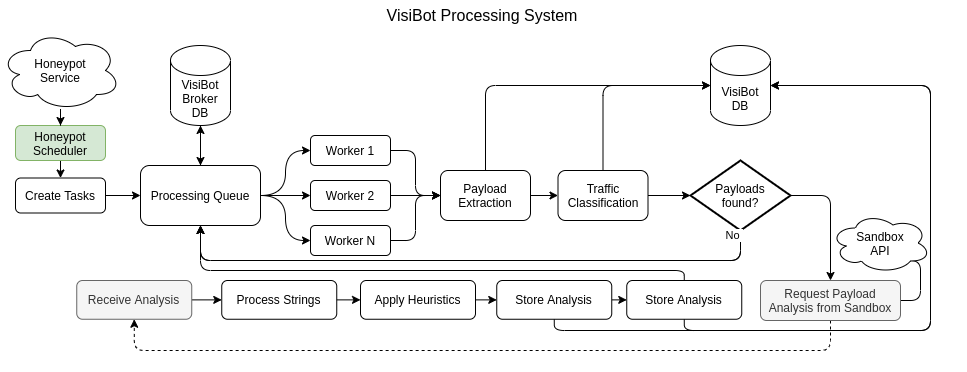
\includegraphics[width=0.9\linewidth]{flowcharts/high_level_processing_overview.png}
    \caption{High-level flow-diagram of the core VisiBot Processing System.}
    \label{fig:high_level_proc_overview} 
\end{figure}

\subsection{Scalable Sandboxing Service}

Like the VisiBot Processing System, the employed sandbox analysis system also utilises the Message Broker architectural design pattern. The VisiBot Processing System's tasks are performed by several scalable and distributable workers, allowing for real-time malware analysis. Hosted on a separate server from VisiBot, all malware samples are stored within a secure block-storage partition separate from the rest of the system. Upon receiving an analysis request from an external source, such as VisiBot, the sandboxing system will attempt to download and analyse a binary from the URL given in the request. If downloaded successfully, the main process will move the binary to a secure block-storage partition with limited file-system permissions, completely separate from the main system. Following this, an analysis task is added to the sandbox broker queue.

When a worker consumes an analysis task, a three-stage analysis process is performed on the binary. The first stage involves static analysis, in which information such as the target CPU architecture, endianess, and source-code strings of the binary is extracted. Following this, the binary is copied to a virtual machine instance running an embedded Linux operating system. The image used by the Virtual Machine (VM) is selected based on the detected CPU architecture of the binary. Several CPU architectures are supported, including MIPS, ARM, i386, aarch64, and x86/64, all of which are common to targeted IoT devices. Once a new Virtual Machine instance is created, the malware binary is executed and monitored for 30 seconds, after which the virtual machine is reset. During the monitoring procedure, dynamic and network analysis are performed, logging all incoming and outgoing network traffic, processes opened files, and system calls generated by the malware sample. This information is used to create and send a report to the VisiBot Processing System following task completion. The report includes various relevant static, dynamic, and network information, including port usage statistics, DNS queries, HTTP requests, and hard-coded binary strings. Additionally, the sandbox also generates log and pcap files which can be used for further analysis. 

\begin{figure}[!htb]
    \centering
    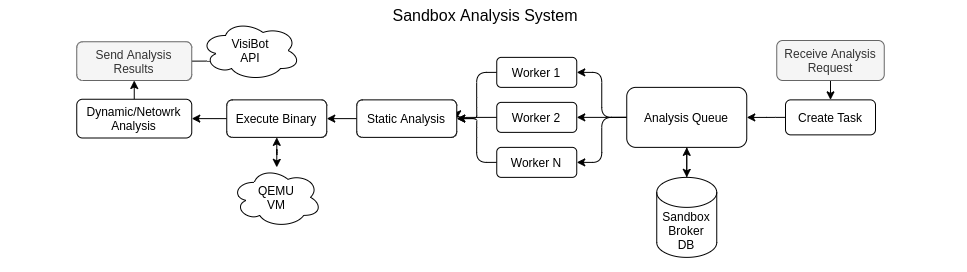
\includegraphics[width=0.9\linewidth]{flowcharts/high_level_sandbox_overview.png}
    \caption{High-level flow-diagram of malware sandbox analysis system.}
    \label{fig:high_level_sandbox} 
\end{figure}

\subsection{Heuristic Analysis}

Once VisiBot receives a malware analysis report from the sandboxing service, heuristic analysis is performed on the sample report to identify candidate Command \& Control servers and Peer-to-Peer botnet activity, similarly to that of \citet{Bastos2019}, \citet{Ceron2019}, and \citet{Herwig2019}. The first heuristic is concerned with identifying Peer-to-Peer botnet activity by analysing DNS queries performed during network analysis. All logged DNS queries are matched against a list of domain names corresponding to Peer-to-Peer Distributed Hash Table services, including commonly used public services offered by bittorrent.com, transmissionbt.com, and utorrent.com. Modern P2P Botnets, such as Mozi, connect to public DHT services to mask peer-to-peer botnet interactions amongst legitimate peers. Thus, the identification of such public DHT DNS names is ideal for inferring the presence of peer-to-peer botnet traffic. 

The second heuristic considers all transactional interactions with public IP addresses as potential C2/P2P activity. A transaction occurs when bytes are both sent to and received from an endpoint. Such data transactions are significant when identifying botnet traffic, as devices infected with botnet malware often attempt to perform handshakes and download updates/binaries from Command \& Control servers, Payload servers, or peer-to-peer botnet nodes.

The third heuristic combines entities of static and dynamic analysis. If any connections are made to hard-coded IP addresses extracted during static analysis, the associated IP address is deemed a candidate C2 server. Lastly, the fourth heuristic uses external IP blacklist services to infer that any IP address endpoints logged during network analysis previously blacklisted for Command \& Control activity are deemed malicious and are considered potential C2 servers. Once candidate C2 servers and P2P Nodes have been identified, the meta-data for each IP address is stored similarly to that of the first-stage classification process, storing geographical information, ASN records, etc. However, as the above heuristics are limited to the detection of \textit{candidate} botnet servers, all endpoints must be further validated through proper handshake confirmation procedures. This process is yet to be implemented within the VisiBot Processing System. However, the system can be easily extended to do so. The modularity of the system, provided by broker-based task processing, ensures that additional analysis stages can be added to the VisiBot Processing System with ease. For a complete high-level overview of the VisiBot Processing System, including remote sandbox integration, see Appendix \ref{appendix_a0}.


\section{Interactive Web Application}

To allow for real-time visualisation of botnet propagation, geographic distribution, and density, an interactive web-based application is used to display the geographic coordinates of all botnet entities identified within the last 24 hours of monitoring. Using the geographic coordinates collected during IP address meta-data collection, botnet entities are pinned onto a world map, using a specific colour to represent different entities, such as Bots, Report servers, C2 servers, and P2P nodes. A variety of information is sourced directly from the VisiBot database and can be viewed through a front-end web interface that communicates with a back-end web server:

\begin{figure}[!htb]
    \centering
    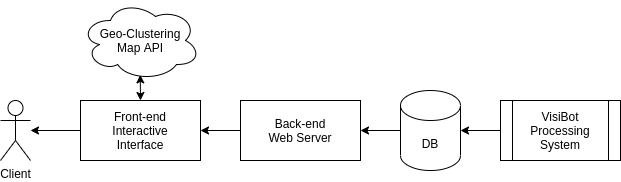
\includegraphics[width=0.7\linewidth]{flowcharts/design_overview_webapp.png}
    \caption{High-level overview of the VisiBot Web Interface.}
    \label{fig:webapp_design_overview} 
\end{figure}

Due to the amount of graphics being re-rendered whenever the map is updated, plotting thousands of geographic coordinates on a single world map can result in high resource usage. A greedy geographic clustering algorithm is used to cluster coordinates into groups based on the geographic distance between points, mitigating visualisation performance issues:

\begin{lstlisting}[caption={Pseudocode for Greedy clustering algorithm based on an example by \citet{MarkerClustering}}]
for each marker:
    if any cluster within cluster_distance of marker
        join(marker, cluster)
    else if any unclustered marker within cluster_distance of marker          create_cluster(marker, unclustered_marker)
\end{lstlisting}

Once clustered, the marker clusters are drawn in the map in place of individual markers. When selected, the map will zoom in and un-cluster markers outside of the specified clustering distance. When a marker is selected, the visitor can view details about the entity and visualise its relationships with other entities recorded by VisiBot.
